%%%%%%%%%%%%%%%%%%%%%%%%%%%%%%%%%%%%%%%%%
% Beamer Presentation
% LaTeX Template
% Version 1.0 (10/11/12)
%
% This template has been downloaded from:
% http://www.LaTeXTemplates.com
%
% License:
% CC BY-NC-SA 3.0 (http://creativecommons.org/licenses/by-nc-sa/3.0/)
%
%%%%%%%%%%%%%%%%%%%%%%%%%%%%%%%%%%%%%%%%%

%----------------------------------------------------------------------------------------
%	PACKAGES AND THEMES
%----------------------------------------------------------------------------------------

\documentclass{beamer}

\mode<presentation> {

% The Beamer class comes with a number of default slide themes
% which change the colors and layouts of slides. Below this is a list
% of all the themes, uncomment each in turn to see what they look like.

%\usetheme{default}
\usetheme{AnnArbor}
%\usetheme{Antibes}
%\usetheme{Bergen}
%\usetheme{Berkeley}
%\usetheme{Berlin}
%\usetheme{Boadilla}
%\usetheme{CambridgeUS}
%\usetheme{Copenhagen}
%\usetheme{Darmstadt}
%\usetheme{Dresden}
%\usetheme{Frankfurt}
%\usetheme{Goettingen}
%\usetheme{Hannover}
%\usetheme{Ilmenau}
%\usetheme{JuanLesPins}
%\usetheme{Luebeck}
%\usetheme{Madrid}
%\usetheme{Malmoe}
%\usetheme{Marburg}
%\usetheme{Montpellier}
%\usetheme{PaloAlto}
%\usetheme{Pittsburgh}
%\usetheme{Rochester}
%\usetheme{Singapore}
%\usetheme{Szeged}
%\usetheme{Warsaw}

% As well as themes, the Beamer class has a number of color themes
% for any slide theme. Uncomment each of these in turn to see how it
% changes the colors of your current slide theme.

%\usecolortheme{albatross}
%\usecolortheme{beaver}
%\usecolortheme{beetle}
\usecolortheme{crane}
%\usecolortheme{dolphin}
%\usecolortheme{dove}
%\usecolortheme{fly}
%\usecolortheme{lily}
%\usecolortheme{orchid}
%\usecolortheme{rose}
%\usecolortheme{seagull}
%\usecolortheme{seahorse}
%\usecolortheme{whale}
%\usecolortheme{wolverine}

%\setbeamertemplate{footline} % To remove the footer line in all slides uncomment this line
%\setbeamertemplate{footline}[page number] % To replace the footer line in all slides with a simple slide count uncomment this line

%\setbeamertemplate{navigation symbols}{} % To remove the navigation symbols from the bottom of all slides uncomment this line
}

\usepackage[utf8]{inputenc}
\usepackage[russian]{babel}
\usepackage{wrapfig}

\usepackage{graphicx} % Allows including images
\usepackage{booktabs} % Allows the use of \toprule, \midrule and \bottomrule in tables

%----------------------------------------------------------------------------------------
%	TITLE PAGE
%----------------------------------------------------------------------------------------

\title[Алгебраические преобразования $\sigma$-матриц]{Алгебраические   преобразования   произведений   скалярных   и   смешанных   произведений
матриц Паули} % The short title appears at the bottom of every slide, the full title is only on the title page

\author[Филипп Усков]{Филипп Усков\\[2mm]Елена Шпагина, Олег Лычковский, Николай Ильин} % Your name
\institute[Сколтех] % Your institution as it will appear on the bottom of every slide, may be shorthand to save space
{
Сколтех; МГУ им. Ломоносова \\ % Your institution for the title page
\medskip
\textit{fel1992@mail.ru} % Your email address
}
\date{\today} % Date, can be changed to a custom date

\begin{document}

\begin{frame}
\titlepage % Print the title page as the first slide
\end{frame}

\begin{frame}
\frametitle{Содержание} % Table of contents slide, comment this block out to remove it
\tableofcontents % Throughout your presentation, if you choose to use \section{} and \subsection{} commands, these will automatically be printed on this slide as an overview of your presentation
\end{frame}

%----------------------------------------------------------------------------------------
%	PRESENTATION SLIDES
%----------------------------------------------------------------------------------------

%------------------------------------------------
%\section{Оценка энергии основного состояния систем с гайзенберговским взаимодействием}
% Sections can be created in order to organize your presentation into discrete blocks, all sections and subsections are automatically printed in the table of contents as an overview of the talk
%\subsection{Оценка сверху} 
% A subsection can be created just before a set of slides with a common theme to further break down your presentation into chunks
%------------------------------------------------

\newcommand{\ssigma}{{\boldsymbol{\sigma}}}
\newcommand{\cc}{{\boldsymbol{\sigma}}}
\newcommand{\tr}{\mathrm{tr}}

%------------------------------------------------
\section{Оценка энергии основного состояния снизу}% систем с гайзенберговским взаимодействием}
%------------------------------------------------
%слайд с мотивацией и рассказом, что такое ск. и смешанное произведение
\begin{frame}
\frametitle{Системы с гайзенберговским взаимодействием}
\begin{wrapfigure}{l}{0.3\textwidth}
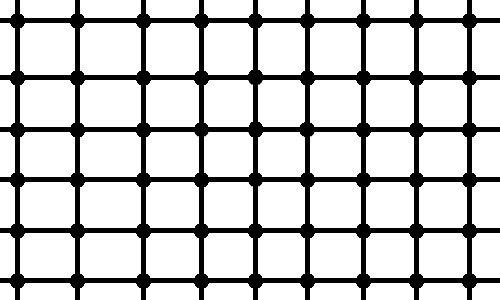
\includegraphics[width=0.3\textwidth]{lattice.png}
\end{wrapfigure}

\begin{center}Типичный Гамильтониан:\end{center}
$$H=\sum_{<i,j>}(\cc_i \cc_j)$$

$<i,j>$ - соседние чатицы в решётке

%\vspace{1em}

%$$\min_{|\psi\rangle}\langle\psi|H|\psi\rangle = E_{gs}$$

%\vspace{1em}

%Задача: $E_{gs}>?$

%\vspace{1em}

Скалярное произведение: 

$(\cc_1\cc_3) = (\cc_3\cc_1) = \sigma_1^\alpha\otimes 1_2\otimes\sigma_3^\alpha \otimes 1_4 \otimes 1_5 $% = 
%$\sigma^x\otimes 1\otimes\sigma^x+\sigma^y\otimes 1\otimes\sigma^y+\sigma^z\otimes 1\otimes\sigma^z$

Смешанное произведение 

$(\cc_1\cc_3\cc_4) = 
\varepsilon^{\alpha\beta\gamma} \times \sigma_1^\alpha\otimes 1_2\otimes\sigma_3^\beta\otimes \sigma_4^\gamma \otimes 1_5 $

$\alpha,\beta,\gamma \in \{x,y,z\}$

\end{frame}

%------------------------------------------------
%\subsection{Оценка сверху} 
%------------------------------------------------
%слайд
%------------------------------------------------
\subsection{через энергию основного состояния подсистем}
%------------------------------------------------
%слайд по Тарраху Валенти => решение УШ
\begin{frame}
\frametitle{Оценка через энергию основного состояния подсистем}
\begin{wrapfigure}{l}{0.3\textwidth}
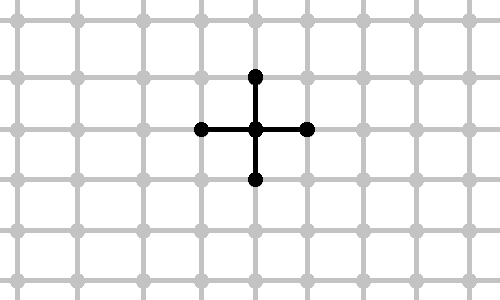
\includegraphics[width=0.3\textwidth]{lattice-crest.png}
\end{wrapfigure}

$$H=\sum_i H_i \quad \Rightarrow \quad E_{gs}\geqslant\sum_i E_{{gs}_i}$$

Для квадратной решетки, которую можем замостить одинаковыми кластерами:
$$E_{gs}/N \geqslant \frac{2}{M}E_{gs_C}$$
где $E_{gs}/N$ - энергия основного состояния решетки, приходящаяся на 1 спин

$M$ - число связей в кластере

$E_{gs_C}$ - энергия основного состояния клатера
\footnotesize{
\begin{thebibliography}{99}
\bibitem[TV, 1990]{TV} R.~Tarrah, R.~Valenti (1990)
\newblock Exact lover bounds to the ground state of spin systems: The two-dimensional $S=\frac12$ antiferromagnetic Geisenberg model
\newblock \emph{Physical rewiew B} , 1990.
\end{thebibliography}
}
\end{frame}
%------------------------------------------------
\subsection{через вариационный метод}
%------------------------------------------------
%слайд по Лычковскому и Ко => квадратичная параметризация
\begin{frame}
\frametitle{Оценка через вариационный метод}
\begin{wrapfigure}{l}{0.3\textwidth}
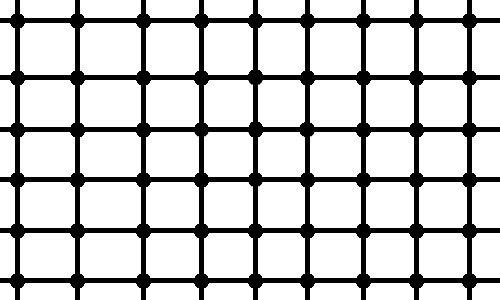
\includegraphics[width=0.3\textwidth]{lattice.png}
\end{wrapfigure}

Для квадратной решетки, которую можем замостить одинаковыми кластерами:
\vspace{1em}

$$E_{gs}/N \geqslant \frac{2}{M}\min_{\rho_c}\tr \,H_c\rho_c$$

\vspace{1em}
где $E_{gs}/N$ - энергия основного состояния системы, приходящаяся на 1 спин

$M$ - число связей в кластере

$H_c,\;\rho_c$ - гамильтониан и матрица плотности клатера 

\footnotesize{
\begin{thebibliography}{99}
\bibitem{hroero}
David A. Mazziotti
\newblock Advances in Chemical Physics, Reduced-Density-Matrix Mechanics: With Application to Many-Electron Atoms and Molecules
\newblock {\em Volume 134. Wiley-Interscience, 1 edition.}, 2007.
\end{thebibliography}
}

\end{frame}
%------------------------------------------------
\section{базис матриц плотности}
%------------------------------------------------
\subsection{Учет симметрий и создание базиса}
%------------------------------------------------
%слайд
\begin{frame}
\frametitle{Учет симметрий и создание базиса}
т.к. гамильтониан обладает \textbf{ вращательной симметрией}, то матрица плотности тоже должна быть вращательно инвариантна

а значит должна состоять из \textbf{ скалярных и смешанных произведений} $\sigma$-матриц

т.к. гамильтониан обладает \textbf{симметрией обращения по времени} $T[H]=H$, и $T[\cc]=-\cc$

то матрица плотности должна состоять \textbf{только из скалярных произведений} $\sigma$-матриц

$$\rho=\frac{1}{2^N}\left(1+a_{i,j}(\ssigma_i \ssigma_j)+b_{i,j,k,l}(\ssigma_i \ssigma_j)(\ssigma_k \ssigma_l)+...\right)$$

Также можно ввести скалярное произведение на этом базисе: $(A,B)=\tr A B, \qquad A^+=A, \qquad \tr( a\otimes b \otimes c) = (\tr a)(\tr b)(\tr c)$

тогда базис можно назвать ортогональным (почти)
\end{frame}

%------------------------------------------------
\begin{frame}
\frametitle{Линейная независимость элементов базиса}
\small
$$\begin{gathered}(\cc_1\cc_2)(\cc_3\cc_4)\;(\cc_1\cc_3)(\cc_2\cc_4) = 
3-2 (\cc_1\cc_2)-2 (\cc_1\cc_3)+2 (\cc_1\cc_4)+2 (\cc_2\cc_3)-\\
-2 (\cc_2\cc_4)+(\cc_1\cc_3) (\cc_2\cc_4)-2 (\cc_3\cc_4)+(\cc_1\cc_2) (\cc_3\cc_4)+\\+i (\cc_1\cc_2\cc_3)-i (\cc_1\cc_2\cc_4)+i (\cc_1\cc_3\cc_4)-i (\cc_2\cc_3\cc_4)\end{gathered}$$

\begin{columns}[c] % The "c" option specifies centered vertical alignment while the "t" option is used for top vertical alignment
\column{.35\textwidth}
$$A=(\cc_1\cc_2)(\cc_3\cc_4)$$
$$B=(\cc_1\cc_3)(\cc_2\cc_4)$$
$$C=(\cc_1\cc_4)(\cc_2\cc_3)$$

\column{.65\textwidth}
$$
\begin{pmatrix}
(AA)&(AB)&(AC)\\
(BA)&(BB)&(BC)\\
(CA)&(CB)&(CC)
\end{pmatrix}
=
\begin{pmatrix}
9&3&3\\
3&9&3\\
3&3&9
\end{pmatrix}
> 0
$$
\end{columns}
\normalsize
\end{frame}
%------------------------------------------------
\begin{frame}
\frametitle{Линейная независимость элементов базиса}
\tiny
\begin{columns}[c] % The "c" option specifies centered vertical alignment while the "t" option is used for top vertical alignment
\column{.25\textwidth}
$$\begin{gathered}
(\cc_1\cc_4) (\cc_2\cc_5) (\cc_3\cc_6)\\
(\cc_1\cc_4) (\cc_2\cc_6) (\cc_3\cc_5)\\
(\cc_1\cc_5) (\cc_2\cc_4) (\cc_3\cc_6)\\
(\cc_1\cc_5) (\cc_2\cc_6) (\cc_3\cc_4)\\
(\cc_1\cc_6) (\cc_2\cc_4) (\cc_3\cc_5)\\
(\cc_1\cc_6) (\cc_2\cc_5) (\cc_3\cc_4)\\
(\cc_1\cc_3) (\cc_2\cc_5) (\cc_4\cc_6)\\
(\cc_1\cc_3) (\cc_2\cc_6) (\cc_4\cc_5)\\
(\cc_1\cc_5) (\cc_2\cc_3) (\cc_4\cc_6)\\
(\cc_1\cc_6) (\cc_2\cc_3) (\cc_4\cc_5)\\
(\cc_1\cc_3) (\cc_2\cc_4) (\cc_5\cc_6)\\
(\cc_1\cc_4) (\cc_2\cc_3) (\cc_5\cc_6)\\
(\cc_1\cc_2) (\cc_3\cc_5) (\cc_4\cc_6)\\
(\cc_1\cc_2) (\cc_3\cc_6) (\cc_4\cc_5)\\
(\cc_1\cc_2) (\cc_3\cc_4) (\cc_5\cc_6)
\end{gathered}$$
\column{.75\textwidth}
$$
\begin{bmatrix}
27& 9& 9& 3& 3& 9& 9& 3& 3& 3\\
9& 27& 3& 9& 9& 3& 3& 9& 3& 3\\
9& 3& 27& 9& 9& 3& 3& 3& 9& 3\\
3& 9& 9& 27& 3& 9& 3& 9& 9& 3\\
3& 9& 9& 3& 27& 9& 3& 3& 3& 9\\
9& 3& 3& 9& 9& 27& 9& 3& 3& 9\\
9& 3& 3& 3& 3& 9& 27& 9& 9& 3\\
3& 9& 3& 9& 3& 3& 9& 27& 3& 9\\
3& 3& 9& 9& 3& 3& 9& 3& 27& 9\\
3& 3& 3& 3& 9& 9& 3& 9& 9& 27\\
3& 3& 9& 3& 9& 3& 9& 9& 3& 3\\
9& 9& 3& 3& 3& 3& 3& 3& 9& 9\\
3& 9& 3& 3& 9& 3& 9& 3& 9& 3\\
9& 3& 9& 3& 3& 3& 3& 9& 3& 9\\
3& 3& 3& 9& 3& 9& 3& 3& 3& 3
\end{bmatrix}
\begin{bmatrix}
 3& 9& 3& 9& 3\\
 3& 9& 9& 3& 3\\
 9& 3& 3& 9& 3\\
 3& 3& 3& 3& 9\\
 9& 3& 9& 3& 3\\
 3& 3& 3& 3& 9\\
 9& 3& 9& 3& 3\\
 9& 3& 3& 9& 3\\
 3& 9& 9& 3& 3\\
 3& 9& 3& 9& 3\\
27& 9& 3& 3& 9\\
9& 27& 3& 3& 9\\
3& 3& 27& 9& 9\\
3& 3& 9& 27& 9\\
9& 9& 9& 9& 27
\end{bmatrix}>0$$
\end{columns}
\normalsize
\end{frame}
%------------------------------------------------
\begin{frame}
\frametitle{Линейная зависимость элементов базиса}
\small
\begin{columns}[c] % The "c" option specifies centered vertical alignment while the "t" option is used for top vertical alignment
\column{.25\textwidth}
$$\begin{gathered}
(\cc_1\cc_2) (\cc_3\cc_4\cc_5)\\
(\cc_1\cc_3) (\cc_2\cc_4\cc_5)\\
(\cc_1\cc_4) (\cc_2\cc_3\cc_5)\\
(\cc_1\cc_5) (\cc_2\cc_3\cc_4)\\
(\cc_2\cc_3) (\cc_1\cc_4\cc_5)\\
(\cc_2\cc_4) (\cc_1\cc_3\cc_5)\\
(\cc_2\cc_5) (\cc_1\cc_3\cc_4)\\
(\cc_3\cc_4) (\cc_1\cc_2\cc_5)\\
(\cc_3\cc_5) (\cc_1\cc_2\cc_4)\\
(\cc_4\cc_5) (\cc_1\cc_2\cc_3)
\end{gathered}$$
\column{.75\textwidth}
$$\begin{pmatrix}
18& 6& -6& 6& 6& -6& 6& 0& 0& 0\\
6& 18& 6& -6& 6& 0& 0& -6& 6& 0\\
-6& 6& 18& 6& 0& 6& 0& -6& 0& 6\\
6& -6& 6& 18& 0& 0& 6& 0& -6& 6\\
6& 6& 0& 0& 18& 6& -6& 6& -6& 0\\
-6& 0& 6& 0& 6& 18& 6& 6& 0& -6\\
6& 0& 0& 6& -6& 6& 18& 0& 6& -6\\
0& -6& -6& 0& 6& 6& 0& 18& 6& 6\\
0& 6& 0& -6& -6& 0& 6& 6& 18& 6\\
0& 0& 6& 6& 0& -6& -6& 6& 6& 18
\end{pmatrix}\geqslant 0$$
\end{columns}
\normalsize
\end{frame}
%------------------------------------------------
\subsection{Умножение элементов базиса}
%------------------------------------------------
%слайд с тривиальным алгоритмом
\begin{frame}
\frametitle{алгоритм симв. умножения через тождество Паули}
реализован на \textcolor{red}{wolfram mathematica} и \textcolor{red}{nikhef form}

входные и выходные данные задаются в виде: 

$(\ssigma_i \ssigma_j) = d(i,j) \qquad (\ssigma_i \ssigma_j \ssigma_k) = t(i,j,k)$

(подразумевается, что разные спиновые индексы не могут быть равны)

\begin{enumerate}
\item 
%\item 
$d(i,j)\rightarrow\sigma(i,\alpha)\sigma(j,\alpha)\qquad
t(i,j,k)\rightarrow\varepsilon(\alpha,\beta,\gamma)\sigma(i,\alpha)\sigma(j,\beta)\sigma(k,\gamma)$
\item $\sigma$-матрицы с разными спиновыми индексами коммутируют, так что мы можем их стабильно отсортировать:
например
$$\begin{gathered}
(\sigma(1,\mu)\sigma(3,\mu))(\sigma(1,\alpha)\sigma(3,\beta)\sigma(6,\gamma)\varepsilon(\alpha,\beta,\gamma) = \\
=\sigma(1,\mu,\alpha) \sigma(3,\mu,\beta) \sigma(6,\gamma) \varepsilon(\alpha,\beta,\gamma)
\end{gathered}
$$
\item $\sigma(i,\alpha,\beta,\gamma)=\sigma_i^\alpha \sigma_i^\beta \sigma_i^\gamma.$ Теперь можно применить тождество Паули: 
	$$\sigma(i,\alpha,\beta,\gamma,...)\rightarrow
	\delta(\alpha,\beta)\sigma(i,\gamma,...)+i \varepsilon(\alpha,\beta,\mu)\sigma(i,\mu,\gamma,...)$$
\item теперь все $\sigma$-матрицы коммутируют, можно упростить $\delta$ и $\varepsilon$ символы и выделить $d(i,j)$ и $t(i,j,k)$
\end{enumerate}
\end{frame}
%------------------------------------------------
%слайд с рекурсивными формулами
\begin{frame}
\frametitle{альтернативные базовые соотношения}
которые можно применыть рекурсивно:
\small
\begin{align}
  % d(1,2)^2 =
  %     + 3
  %     - 2*d(1,2)
  (\ssigma_1\ssigma_2)^2 = & \,\,\,  3\
  -2 (\ssigma_1\ssigma_2)				%\label{q1}
  \\
  %
  % d(1,2)*d(2,3) =
  %     - t(1,2,3)*i_
  %     + d(1,3)
  (\ssigma_1\ssigma_2)(\ssigma_2\ssigma_3) = &\
  -i(\ssigma_1\ssigma_2\ssigma_3)\
  +(\ssigma_1\ssigma_3)					%\label{q2}
  \\
  %
  % d(1,2)*t(1,2,3) =
  %     - t(1,2,3)
  %     - 2*d(1,3)*i_
  %     + 2*d(2,3)*i_
  (\ssigma_1\ssigma_2)(\ssigma_1\ssigma_2\ssigma_3) = &\
  -(\ssigma_1\ssigma_2\ssigma_3)\
  -2i(\ssigma_1\ssigma_3)\
  +2i(\ssigma_2\ssigma_3)				%\label{q5}
  \\
  %
  % t(1,2,3)*d(1,2) =
  %     - t(1,2,3)
  %     + 2*d(1,3)*i_
  %     - 2*d(2,3)*i_
  (\ssigma_1\ssigma_2\ssigma_3)(\ssigma_1\ssigma_2) = &\
  -(\ssigma_1\ssigma_2\ssigma_3)\
  +2i(\ssigma_1\ssigma_3)\
  -2i(\ssigma_2\ssigma_3)				%\label{q5a}
  \\
  %
  % d(1,2)*t(2,3,4) =
  %     + t(1,3,4)
  %     - d(1,3)*d(2,4)*i_
  %     + d(1,4)*d(2,3)*i_
  (\ssigma_1\ssigma_2)(\ssigma_2\ssigma_3\ssigma_4) = & \
  (\ssigma_1\ssigma_3\ssigma_4)\
  -i(\ssigma_1\ssigma_3)(\ssigma_2\ssigma_4)\
  +i(\ssigma_1\ssigma_4)(\ssigma_2\ssigma_3)		%\label{q4}
  \\
  %
  % t(2,3,4)*d(1,2) =
  %     + t(1,3,4)
  %     + d(1,3)*d(2,4)*i_
  %     - d(1,4)*d(2,3)*i_
  (\ssigma_2\ssigma_3\ssigma_4)(\ssigma_1\ssigma_2) =  &\
  (\ssigma_1\ssigma_3\ssigma_4)\
  +i(\ssigma_1\ssigma_3)(\ssigma_2\ssigma_4)\
  -i(\ssigma_1\ssigma_4)(\ssigma_2\ssigma_3)		%\label{q4a}
  \\
  %
  % t(1,2,3)^2 =
  %     + 6
  %     - 2*d(1,2)
  %     - 2*d(1,3)
  %     - 2*d(2,3)
  (\ssigma_1\ssigma_2\ssigma_3)^2 = &\,\,\,6\
  -2(\ssigma_1\ssigma_2)\
  -2(\ssigma_1\ssigma_3)\
  -2(\ssigma_2\ssigma_3)				%\label{q3}
  \\
  %
  % t(1,2,3)*t(1,2,4) =
  %     + t(1,3,4)*i_
  %     + t(2,3,4)*i_
  %     - d(1,3)*d(2,4)
  %     - d(1,4)*d(2,3)
  %     + 2*d(3,4)
  (\ssigma_1\ssigma_2\ssigma_3)(\ssigma_1\ssigma_2\ssigma_4) = &\
  +i(\ssigma_1\ssigma_3\ssigma_4)\
  +i(\ssigma_2\ssigma_3\ssigma_4) 		\nonumber\\  & \
  -(\ssigma_1\ssigma_3)(\ssigma_2\ssigma_4) \
  -(\ssigma_1\ssigma_4)(\ssigma_2\ssigma_3)
  +2 (\ssigma_3\ssigma_4)				%\label{q6}
  \\
  %
  % t(1,2,3)*t(1,4,5) =
  %     - d(1,2)*t(3,4,5)*i_
  %     + d(1,3)*t(2,4,5)*i_
  %     + d(2,4)*d(3,5)
  %     - d(2,5)*d(3,4)
  (\ssigma_1\ssigma_2\ssigma_3)(\ssigma_1\ssigma_4\ssigma_5) = & \
  -i(\ssigma_1 \ssigma_2)(\ssigma_3 \ssigma_4 \ssigma_5) \
  +i(\ssigma_1 \ssigma_3 )(\ssigma_2 \ssigma_4 \ssigma_5) \nonumber\\  & \
  +(\ssigma_2 \ssigma_4)(\ssigma_3 \ssigma_5)\
  -(\ssigma_2 \ssigma_5)(\ssigma_3 \ssigma_4) 		%\label{q7}
%  \\
  %
  % d(1,2)*d(2,3)*d(3,4) =
  %     - t(1,2,4)*i_
  %     - t(1,3,4)*i_
  %     + d(1,4)
  %     - d(1,3)*d(2,4)
  %     + d(1,4)*d(2,3)
%  (\ssigma_1\ssigma_2)(\ssigma_2\ssigma_3)(\ssigma_3\ssigma_4) =& \
%  -i(\ssigma_1\ssigma_2\ssigma_4)\
%  -i(\ssigma_1\ssigma_3\ssigma_4)\
%  +(\ssigma_1\ssigma_4)		\nonumber\\&\
%  +(\ssigma_1\ssigma_4)(\ssigma_2\ssigma_3)\
%  -(\ssigma_1\ssigma_3)(\ssigma_2\ssigma_4)		%\label{q8}
%  \\
  %
  % d(1,2)*d(3,4)*d(1,3)*d(2,4) =
  %     + 3
  %     + t(1,2,3)*i_
  %     - t(1,2,4)*i_
  %     + t(1,3,4)*i_
  %     - t(2,3,4)*i_
  %     - 2*d(1,2)
  %     - 2*d(1,3)
  %     + 2*d(1,4)
  %     + 2*d(2,3)
  %     - 2*d(2,4)
  %     - 2*d(3,4)
  %     + d(1,2)*d(3,4)
  %     + d(1,3)*d(2,4)
%  (\ssigma_1\ssigma_2)(\ssigma_3\ssigma_4)(\ssigma_1\ssigma_3)(\ssigma_2\ssigma_4) = & \,\,\,3\
%  +i(\ssigma_1\ssigma_2\ssigma_3)\
%  -i(\ssigma_1\ssigma_2\ssigma_4)\
%  +i(\ssigma_1\ssigma_3\ssigma_4)\
%  -i(\ssigma_2\ssigma_3\ssigma_4)	\nonumber\\&\
%  -2(\ssigma_1\ssigma_2)\
%  -2(\ssigma_1\ssigma_3)\
%  +2(\ssigma_1\ssigma_4)		\nonumber\\&\
%  +2(\ssigma_2\ssigma_3)\
%  -2(\ssigma_2\ssigma_4)\
%  -2(\ssigma_3\ssigma_4)		\nonumber\\&\
%  +(\ssigma_1\ssigma_2)(\ssigma_3\ssigma_4)\
%  +(\ssigma_1\ssigma_3)(\ssigma_2\ssigma_4) 		%\label{q9}
\end{align}
\normalsize

\end{frame}
%------------------------------------------------
\section{Уравнение Шредингера в виде $H\rho=E\rho$}
%------------------------------------------------
%слайд с тремя частицами
%слайд с уравнением и ссылкой
\begin{frame}
\frametitle{Уравнение Шредингера в виде $H\rho=E\rho$ \cite{hroero}}
Рассмотрим пример из 3 частиц
$$H=(\cc_1,\cc_2)+(\cc_2,\cc_3)$$
Гамильтониан обладает дополнительной симметрией: $1\leftrightarrow 3$
$$\rho = \frac18\big(1+a\big((\cc_1,\cc_2)+(\cc_2,\cc_3)\big)+b(\cc_1,\cc_3)\big)$$

\footnotesize{
\begin{thebibliography}{99}
\bibitem[LGC, 2017]{LGC} Lychkovskiy, Oleg and Gamayun, Oleksandr and Cheianov, Vadim (2017)
\newblock Time Scale for Adiabaticity Breakdown in Driven Many-Body Systems and Orthogonality Catastrophe
\newblock \emph{Phys. Rev. Lett.} 119, 200401 (2017).
\end{thebibliography}
}


\end{frame}
%------------------------------------------------
%слайд с тремя частицами
\begin{frame}
\frametitle{пример с тремя частицами}
\small
$$\begin{gathered}
H\rho=\frac18((\cc_1,\cc_2)+(\cc_2,\cc_3)) (1+a((\cc_1,\cc_2)+(\cc_2,\cc_3))+b(\cc_1,\cc_3)) =\\
= \frac18(6 a +(1+b- 2 a) (\cc_1, \cc_2)  + 2 a (\cc_1, \cc_3) +(1+b- 2 a) (\cc_2, \cc_3)) =\\
= \frac18(E+E a(\cc_1,\cc_2)+E a(\cc_2,\cc_3) + E b(\cc_1,\cc_3)) = E\rho
\end{gathered}$$

\begin{columns}[c] % The "c" option specifies centered vertical alignment while the "t" option is used for top vertical alignment

\column{.45\textwidth} % Left column and width
получается система из трех квадратных уравнений

$$
\begin{cases}
6 a-E=0\\
1-2 a+b-a E=0\\
2 a-b E=0
\end{cases}
$$

\column{.5\textwidth} % Right column and width
Решение:

$$
\begin{cases}
a=-\frac12 \\b= \frac13 \\E=-4
\end{cases} \quad
\begin{cases}
a=0 \\b=-1 \\E=0
\end{cases} \quad
\begin{cases}
a=\frac13 \\b=\frac13 \\E=2
\end{cases} \quad
$$

\end{columns}
\normalsize
\end{frame}
%------------------------------------------------
%слайд со скриншотом про крест
\begin{frame}
\frametitle{Применяем для кластера}
\begin{figure}
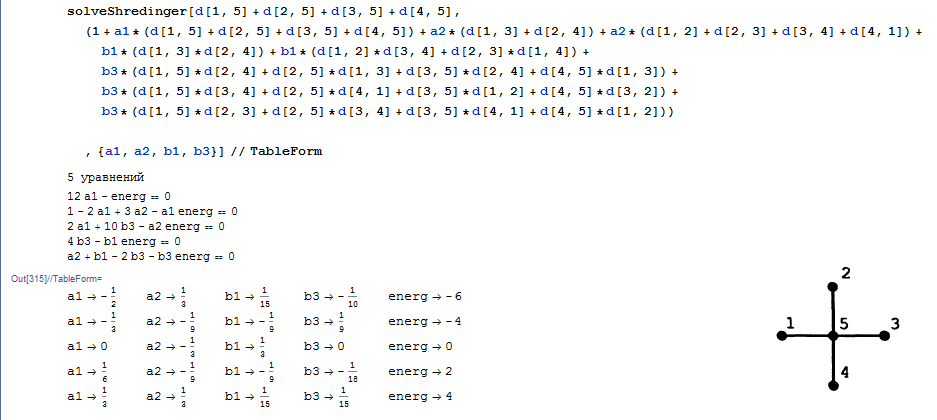
\includegraphics[width=1\linewidth]{solve-crest.png}
\end{figure}
$$E_{gs}/N\geqslant -3$$

\end{frame}
%------------------------------------------------
%слайд про генерацию Ро
\begin{frame}
\frametitle{Алгоритм генерации $\rho$}
... с учетом симметрий гамильтониана - был реализован на \textcolor{red}{wolfram mathematica}
\begin{figure}
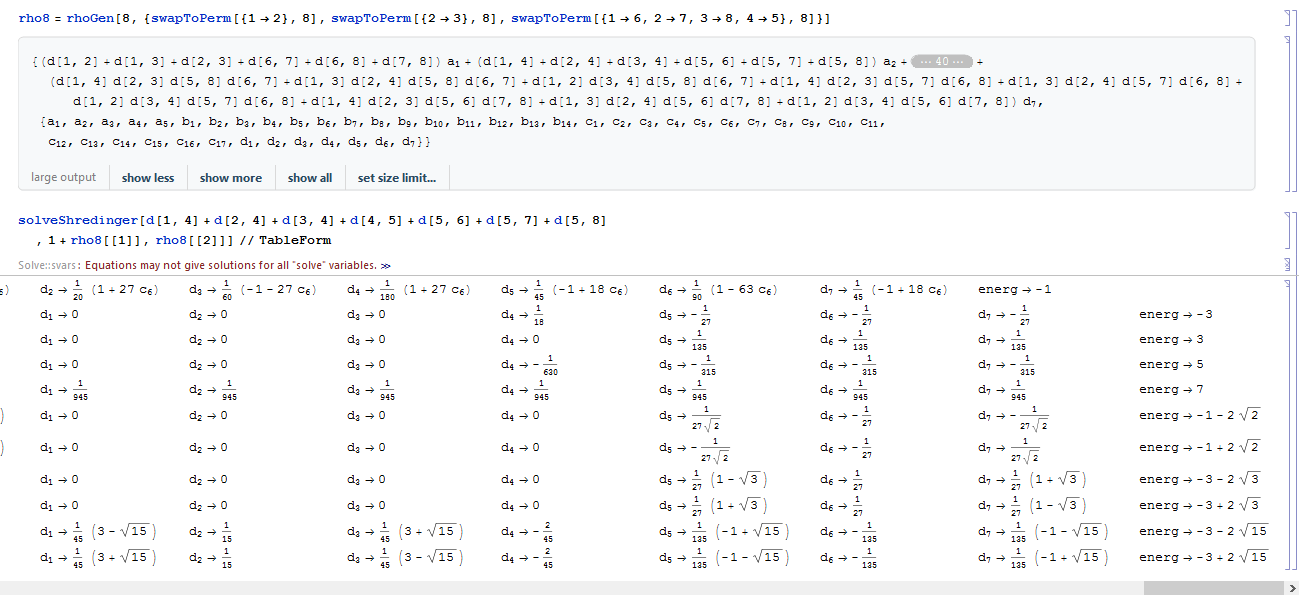
\includegraphics[width=1\linewidth]{result.png}
\end{figure}

\end{frame}
%------------------------------------------------
%слайд про квадратные уравнения и скриншотом про двойной крест
%------------------------------------------------
\section{квадратичная параметризация и поиск минимума}
%------------------------------------------------
%слайд с квадратичной параметризацией
\begin{frame}
\frametitle{Квадратичная параметризация}
Для поиска $\min_\rho \tr H_c\rho_c$ чтобы удовлетворить требованиям 
$$\rho_c \geq 0,\quad \tr \rho_c=1, \quad \rho_c^\dagger=\rho_c$$ 

используется квадратичная параметризация 
$$\rho_c = \frac{\tau^2}{\tr \tau^2}$$

\footnotesize{
\begin{thebibliography}{99}
\bibitem{sqparam}
N.~Il'in, E.~Shpagina, F.~Uskov, O.~Lychkovskiy
\newblock Squaring parametrization of constrained and
  unconstrained sets of quantum states.
\newblock {\em arXiv:1704.03861}.
\end{thebibliography}
}

\end{frame}
%------------------------------------------------
%слайд с применением для кластера
\begin{frame}
\frametitle{пример вар. принципа и кв. параметризации}
с учетом симметрий решетки
\begin{wrapfigure}{r}{0.2\textwidth}
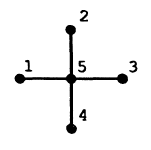
\includegraphics[width=0.2\textwidth]{cluster-crest.png}
\end{wrapfigure}

\small
$$\begin{gathered}
\tau=1 + \\
a_1 ((\cc_1, \cc_5) + (\cc_2, \cc_5) + (\cc_3, \cc_5) + (\cc_4, \cc_5)) + \\
a_2 ((\cc_1, \cc_3) + (\cc_2, \cc_4)) + \\
a_3 ((\cc_1, \cc_2) + (\cc_2, \cc_3) + (\cc_3, \cc_4) + (\cc_4, \cc_1)) + \\
b_1 ((\cc_1, \cc_5) (\cc_2, \cc_3) + (\cc_1, \cc_5) (\cc_4, \cc_3) + (\cc_2, \cc_5) (\cc_3, \cc_4) + (\cc_2, \cc_5) (\cc_1, \cc_4) + \\
+ (\cc_3, \cc_5) (\cc_4, \cc_1) + (\cc_3, \cc_5) (\cc_2, \cc_1) + (\cc_4, \cc_5) (\cc_1, \cc_2) + (\cc_4, \cc_5) (\cc_3, \cc_2)) + \\
b_2 ((\cc_1, \cc_2) (\cc_3, \cc_4) + (\cc_2, \cc_3) (\cc_4, \cc_1)) + \\
b_3 (\cc_1, \cc_3) (\cc_2, \cc_4) + \\
b_4 ((\cc_1, \cc_5) (\cc_2, \cc_4) + (\cc_2, \cc_5) (\cc_1, \cc_3) + (\cc_3, \cc_5) (\cc_2, \cc_4) + (\cc_4, \cc_5) (\cc_1, \cc_3))
\end{gathered}$$

\normalsize
\end{frame}
%------------------------------------------------
\begin{frame}
\frametitle{пример вар. принципа и кв. параметризации}
\small
$$\tr H_c\rho_c = \frac{\begin{gathered}(
24 a_1 - 24 a_1^2 + 24 a_1 a_2 + 48 a_1 a_3 + 48 a_2 b_1 + 192 a_3 b_1 - 192 b_1^2 + 192 b_1 b_2 + \\
48 b_1 b_3 + 72 a_2 b_4 + 48 a_3 b_4 - 96 b_1 b_4 + 48 b_2 b_4 + 72 b_3 b_4 - 72 b_4^2)\end{gathered}}
{1 + 12 a_1^2 + 6 a_2^2 + 12 a_3^2 + 96 b_1^2 + 24 b_2^2 + 12 b_2 b_3 + 9 b_3^2 + 48 b_1 b_4 + 36 b_4^2}$$

$$NMinimize\rightarrow\Bigg\{-6., \begin{cases}
a_1 \rightarrow -0.5,&a_2 \rightarrow 0.333333, \\a_3 \rightarrow 0.333333, \\
b_1 \rightarrow -0.1,&b_2 \rightarrow 0.0666667,\\
b_3 \rightarrow 0.0666667, &b_4 \rightarrow -0.1
\end{cases}\Bigg\} \quad\Rightarrow\quad
E_{gs}/N\geqslant -3
$$
\normalsize
Те же результаты были получены через уравнение Шредингера.

Мы ожидаем, что этот метод превзойдет метод через УШ.

\end{frame}

%------------------------------------------------

\begin{frame}
\frametitle{Литература}
\footnotesize{
\begin{thebibliography}{99}

\bibitem{sqparam}
N.~Il'in, E.~Shpagina, F.~Uskov, O.~Lychkovskiy
\newblock Squaring parametrization of constrained and
  unconstrained sets of quantum states.
\newblock {\em arXiv:1704.03861}.

\bibitem{hroero}
Lychkovskiy, Oleg and Gamayun, Oleksandr and Cheianov, Vadim
\newblock Time Scale for Adiabaticity Breakdown in Driven Many-Body Systems and Orthogonality Catastrophe
\newblock {\em Phys. Rev. Lett. 119},200401 (2017).

\bibitem{VarPr}
David A. Mazziotti
\newblock Advances in Chemical Physics, Reduced-Density-Matrix Mechanics: With Application to Many-Electron Atoms and Molecules
\newblock {\em Volume 134. Wiley-Interscience, 1 edition.}, 2007.

\bibitem{TarrahValenti}
R.~Tarrah and R.~Valenti
\newblock Exact lower bounds to the ground-state energy of spin systems: The two-dimensional $S=\frac12$ antiferromagnetic Heisenberg model
\newblock {\em Physical review B}, 1990.

\end{thebibliography}
}
\end{frame}

%------------------------------------------------

\begin{frame}
\Huge{\centerline{Спасибо за внимание}}
\end{frame}

%----------------------------------------------------------------------------------------

\end{document}